% ****** Start of file aipsamp.tex ******
%
%   This file is part of the AIP files in the AIP distribution for REVTeX 4.
%   Version 4.1 of REVTeX, October 2009
%
%   Copyright (c) 2009 American Institute of Physics.
%
%   See the AIP README file for restrictions and more information.
%
% TeX'ing this file requires that you have AMS-LaTeX 2.0 installed
% as well as the rest of the prerequisites for REVTeX 4.1
%
% It also requires running BibTeX. The commands are as follows:
%
%  1)  latex  aipsamp
%  2)  bibtex aipsamp
%  3)  latex  aipsamp
%  4)  latex  aipsamp
%
% Use this file as a source of example code for your aip document.
% Use the file aiptemplate.tex as a template for your document.
\documentclass[%
aip,
jmp,%
amsmath,amssymb,
preprint,%
reprint,%
notitlepage,
a4paper]{revtex4-1}
\usepackage{natbib}
\usepackage[utf8]{inputenc}
\usepackage{graphicx}% Include figure files
\usepackage{dcolumn}% Align table columns on decimal point
\usepackage{bm}% bold math
\usepackage[mathlines]{lineno}% Enable numbering of text and display math
%\linenumbers\relax % Commence numbering lines
\usepackage[spanish, english]{babel}
\usepackage{float}
\usepackage{rotating}
\usepackage{afterpage}
\usepackage{capt-of}
\usepackage{hyperref}
\usepackage{mathtools}
\usepackage{physics}
\usepackage{siunitx}

\bibliographystyle{aipauth4-1}
\newcommand{\md}{\texttt{md1}}
\newcommand{\average}[1]{\langle #1 \rangle}


\begin{document}
	
	%\preprint{AIP/123-QED}
	
	\title[Computer Simulation of Physical Systems]{Molecular Dynamics of Liquid Argon}% Force line breaks with \\
	
	\author{Daniel Felipe Forero Sánchez}
	\altaffiliation{Section de Physique, LASTRO, EPFL}%Lines break automatically or can be forced with \\
	
	
	\date{\today}% It is always \today, today,
	%  but any date may be explicitly specified
		%display desired

	
	\begin{abstract}
		

	\end{abstract}


	\maketitle

	
	\section{Introduction}
	Molecular dynamics simulations have been fundamental tools in science since they allow for the detailed analysis of various properties of the system that are impossible to probe experimentally. However, to properly simulate a physical system is a complex problem on its own, owing to the size of such systems. Molecular dynamics treats the system as a collection of particles evolving according to the Lennard-Jones potential \cite{Jones1924}; it can be then regarded as a simulation from ``first principles''. To track the position and velocities of $10^{23}$ particles is, in practice, impossible. In such a limit one often uses emergent models such as fluid dynamics. Nonetheless, it is possible to properly model a small physical system with MD and make it an accurate reproduction of the real world \cite{Rahman1964}
\section{Theory}
\subsection{The Lennard-Jones potential}
The Lennard-Jones potential \cite{Jones1924} is commonly used to define the weak interatomic interactions in fluids. It is defined as
\begin{equation}
U(r_{ij}) = 4\epsilon\left[\left(\frac{\sigma}{r_{ij}}\right)^{12} - \left(\frac{\sigma}{r_{ij}}\right)^{6}\right],
\label{eq:lennardjones}
\end{equation}
where $r_{ij} \equiv \norm{\vb{r}_i - \vb{r}_j}$ is the distance between two particles at positions $\vb{r}_{i,j}$. It depends on the constants $\epsilon$ and $\sigma$, which define the energy and length scale of the system, respectively.
\subsection{The Radial distribution function}
The \textit{Radial distribution function} (RDF) is defined as
\begin{equation}
g(r) = \frac{\rho(r)}{\rho_0},
\end{equation}
where $\rho_0 = N/V$ is the constant average density (total number of particles over total volume of the system) and $\rho(r)$ is the density of particles at a distance $r$. The function $g(r)$ is interpreted as the probability of finding a pair of particles separated by a given distance $r$. The RDF is also known as the pair-correlation function. These correlators are ubiquitous in physics and the RDF has analogous quantities in other fields such as cosmology (see cosmological two-point correlation function $\xi(s)$\cite{Peebles1980}). This is not surprising since they encode relevant statistical information about the system (see section \ref{sec:structurefactor}).\\
\subsection{The Structure factor \label{sec:structurefactor}}
The \textit{Structure factor} $S(k)$ is a fundamental quantity in the study of matter, since it can be experimentally measured through scattering experiments\cite{Simon2013}. More importantly, it encodes relevant physical information given that it is closely related to physical quantities such as the scattering potential.\\
Furthermore, $S(k)$ is directly related to $g(r)$ through a Fourier transform:
\begin{equation}
S(k) = 1 + 4\pi\rho_0\int_{\mathbb{R}^+}r^2 [g(r) - 1] \frac{\sin kr}{kr} dr.
\end{equation}
We expect then, that the peaks in $S(k)$ are located at $k\sim 2\pi/s$ with $s$ the typical separation of particles in the system.\\
Following the analogy with cosmology, the structure factor is analogous to the cosmological power spectrum $P(k)$ measured, for example, in the CMB\cite{Peebles1980}.
\subsection{The Diffusion coefficient}
The diffusion equation
\begin{equation}
\dot{C}(\vb{r}, t) = D\nabla^2C(\vb{r}, t),
\label{eq:diffeq}
\end{equation}
describes the evolution of the concentration, $C$, of a substance. The parameter $D$ is the \textit{diffusion coefficient} and defines how fast the substance will diffuse in the media. The kernel of equation \ref{eq:diffeq} is a Gaussian distribution with $\sigma_r^2 = 6Dt$ and $\langle r\rangle=0$, so to compute the diffusion coefficient we compute the second moment of the distribution $C(\vb{r})$, $\langle r^2\rangle$. This yields the Einstein relation\cite{Einstein1905}
\begin{equation}
\pdv{t}\langle r^2\rangle = 6D.
\end{equation}
It is then possible to measure the diffusion coefficient from the \textit{mean square displacement} (MSD) via the relations \ref{eq:diffeinstein}, \ref{eq:msd}.
\begin{align}
\label{eq:diffeinstein}
D =& \lim_{t\rightarrow\infty} \frac{1}{6t}\langle\norm{\Delta\vb{r}(t)}^2\rangle\\
\label{eq:msd}
\langle\norm{\Delta\vb{r}(t)}^2\rangle =& \frac{1}{N}\sum_{i = 1}^{N}\norm{ \vb{r}_i(t) - \vb{r}_i(0)}^2
\end{align}
We can alternatively use the \textit{velocity autocorrelation function} (VACF)\cite{Kubo1957}
\begin{align}
\label{eq:diffvacf}
&D = -\frac{1}{3}\int_{\mathbb{R}^+}\dd{\tau} \langle \vb{v}(\tau)\dotproduct\vb{v}(0)\rangle,\\
&\average{\vb{v}(\tau)\dotproduct\vb{v}(0)} = \sum_{i = 1}^N \vb{v}(\tau)\dotproduct\vb{v}(0)
\end{align}
\section{Methods}
\subsection{Grid Integration}
This kind of integration algorithms rely on space discretization of space and time coordinates, that is, they work on a grid. While there are a great variety of similar integration methods, each one having advantages and disadvantages, we focus on the one used by the \md  code \cite{Ercolessi}. This particular implementation in \texttt{FORTRAN90}, uses the \textit{velocity Verlet} integration algorithm \cite{Swope1982}. This second order method has the following update rules:
\begin{align}
r_{n+1} =& r_n + h v_n + h^2\frac{f(t_n)}{2m},\\
v_{n+1} = & v_n + h\frac{f(t_{n+1} )+ f(t_n)}{2m},
\end{align}
where $r_n$ and $v_n$ define, respectively, the position and velocity at time $t_n\equiv nh$, $h$ is the time step, $f$ is the force $m\ddot{r}_n = f(t_n)$ and $m$, the mass.\\
This algorithm was used to integrate the equations of motion of $N$ particles in the simulation.
\subsection{Monte-Carlo}
\section{The simulations}
\subsection{Liquid Argon}
Rahman\cite{Rahman1964} studied the properties of a liquid Argon system consisting of $N=864$ atoms in a box of length $L = \SI{34.8}{\AA} = 10.229\sigma$. The system was at temperature $T = \SI{94.4}{\kelvin}$ and had a density $\rho_0 = \SI{1.374}{\gram\per\cubic\centi\meter}$. In this simulation, Argon atoms of mass $M = \SI{6.69e-26}{\kilogram}$ interact through the potential shown in equation \ref{eq:lennardjones} with parameters $\epsilon/k_b = \SI{120}{\kelvin}$ and $\sigma = \SI{3.4}{\AA}$. Additionally, the interaction range was cut-off at $R = 2.25\sigma$, while periodic boundary conditions in all directions were assumed. Finally, the time step is defined $h = \SI{1e-2}{\pico\second}$.
\subsection{MD1 code}
EXPLAIN THE STEPS THAT HAVE TO BE TAKEN. INITIALISATION OF THE POSITIONS AND VELOCITIES, CHANGING THE TEMPERATURE AND STABILIZING THE TEMPERATURE (EQUILIBRIUM RUN)
\section{Results}
As a check of the simulation temperature, we study the temperature of the system, shown in figure \ref{fig:Tvst} 
\begin{figure}[t]
	\centering
	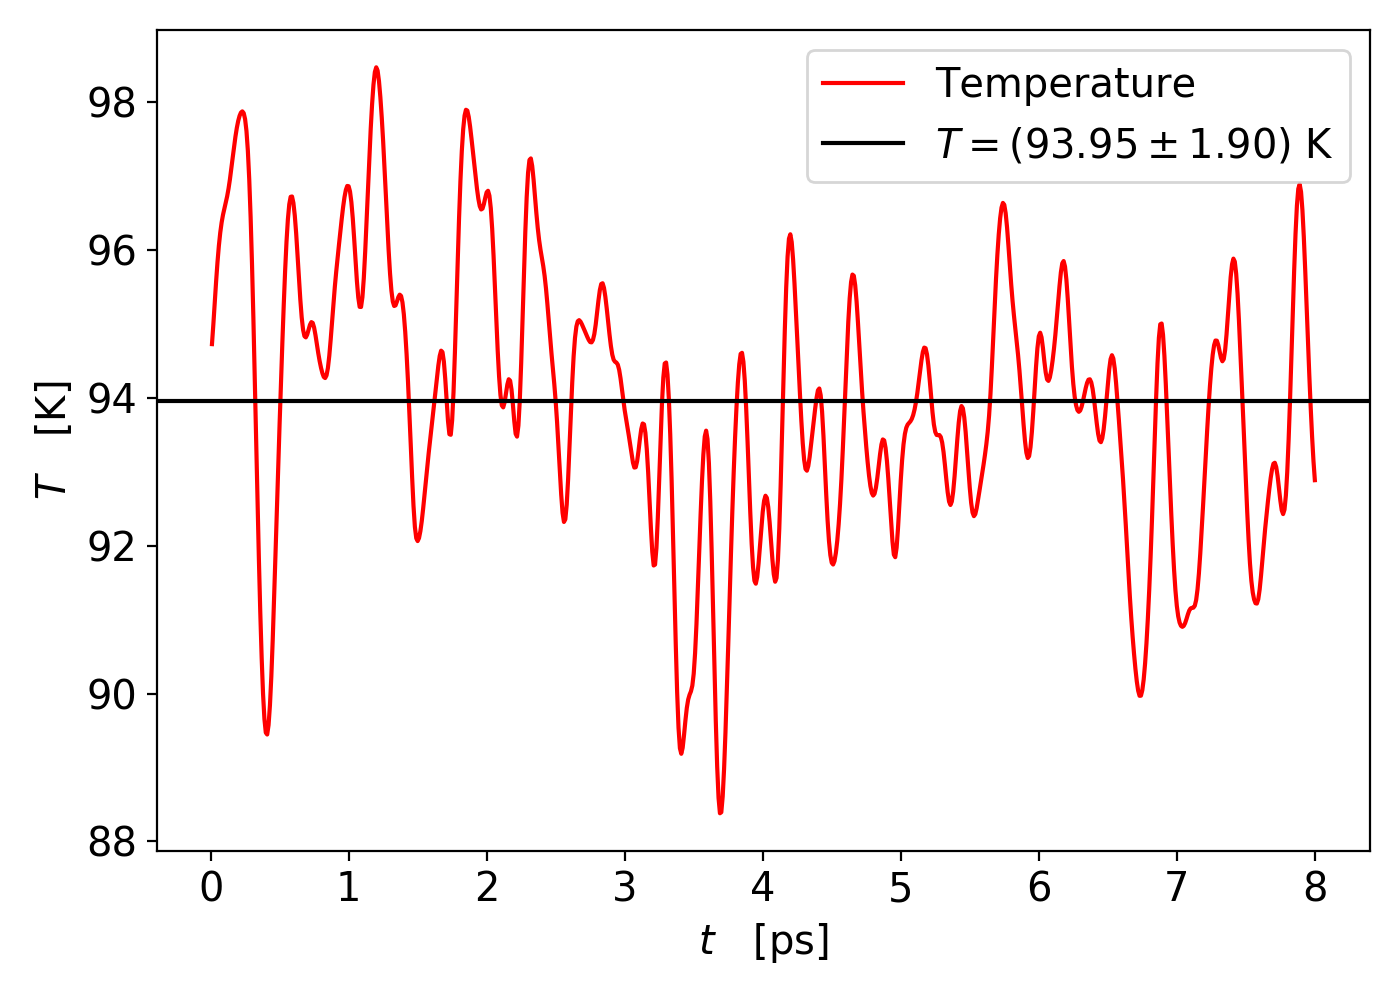
\includegraphics[width=0.9\linewidth]{../task2/results/Tvst}
	\caption{Temperature of the stabilized system.}
	\label{fig:Tvst}
\end{figure}
\subsection{Radial distribution function}
\begin{figure}[t]
	\centering
	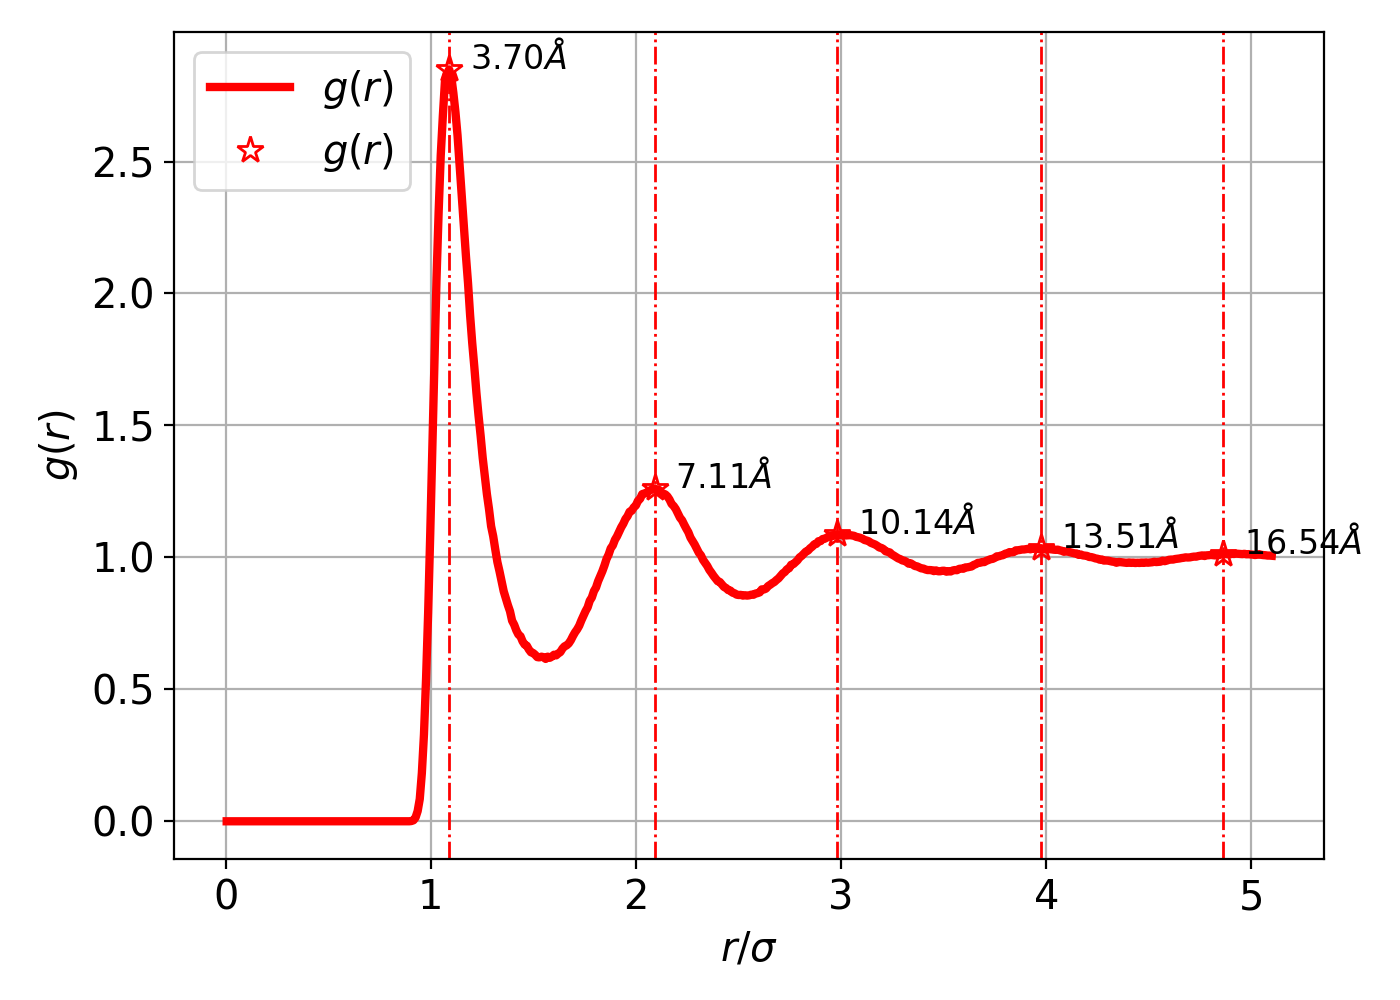
\includegraphics[width=0.9\linewidth]{../task2/results/gofr}
	\caption{Radial distribution function.}
	\label{fig:gofr}
\end{figure}
Figure \ref{fig:gofr} shows the computed 
\subsection{Structure factor}
\begin{figure}
	\centering
	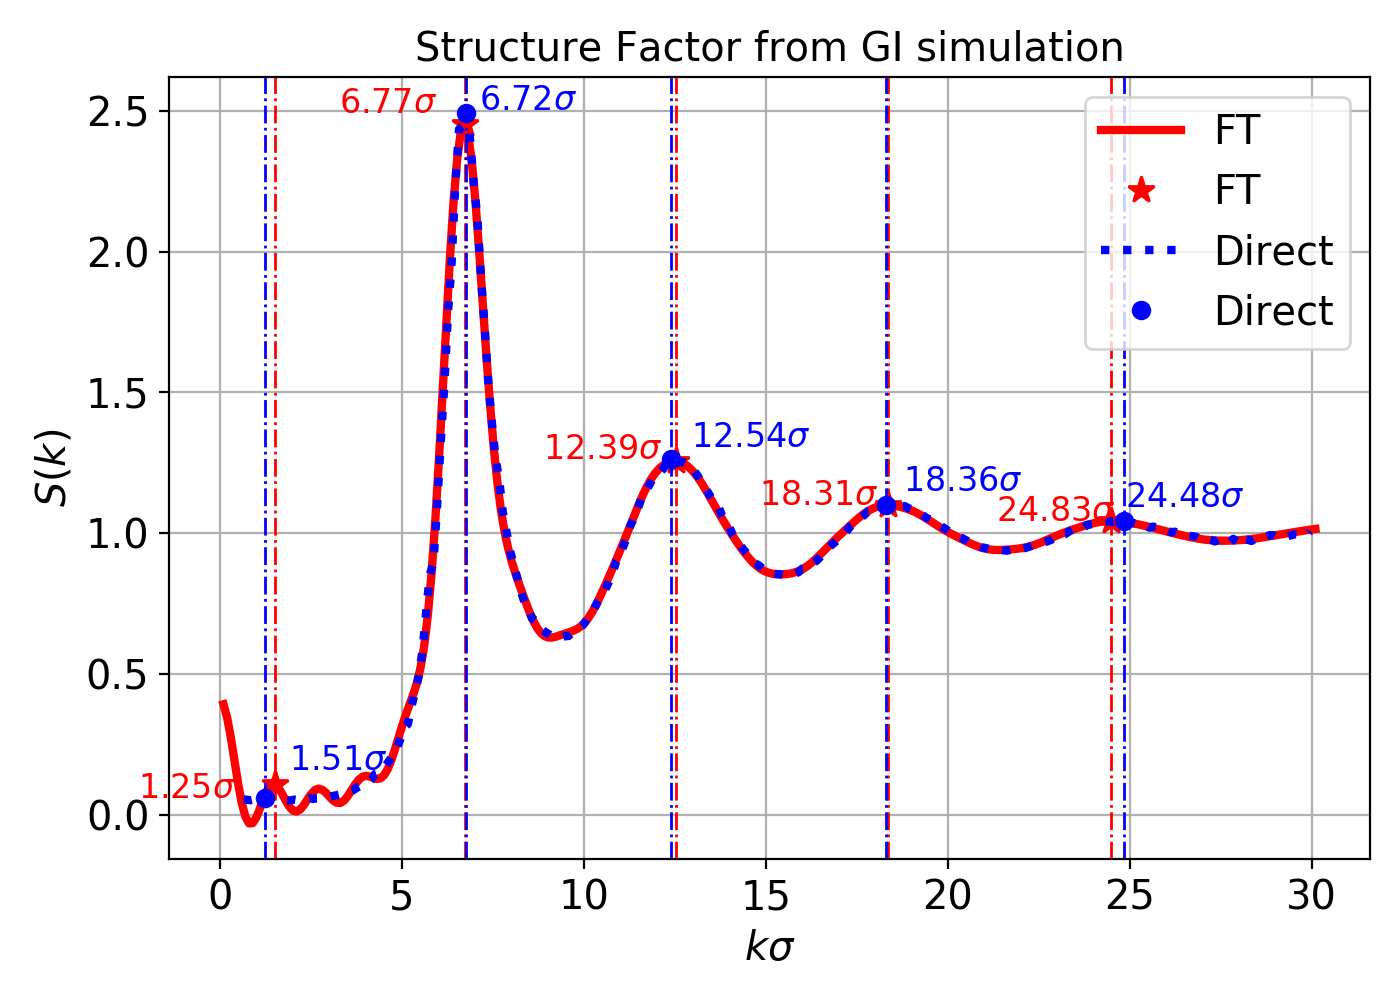
\includegraphics[width=0.9\linewidth]{../task2/results/sofk}
	\caption{Structure factor.}
	\label{fig:sofk}
\end{figure}

\subsection{Diffusion Coefficient}
\begin{figure}
	\centering
	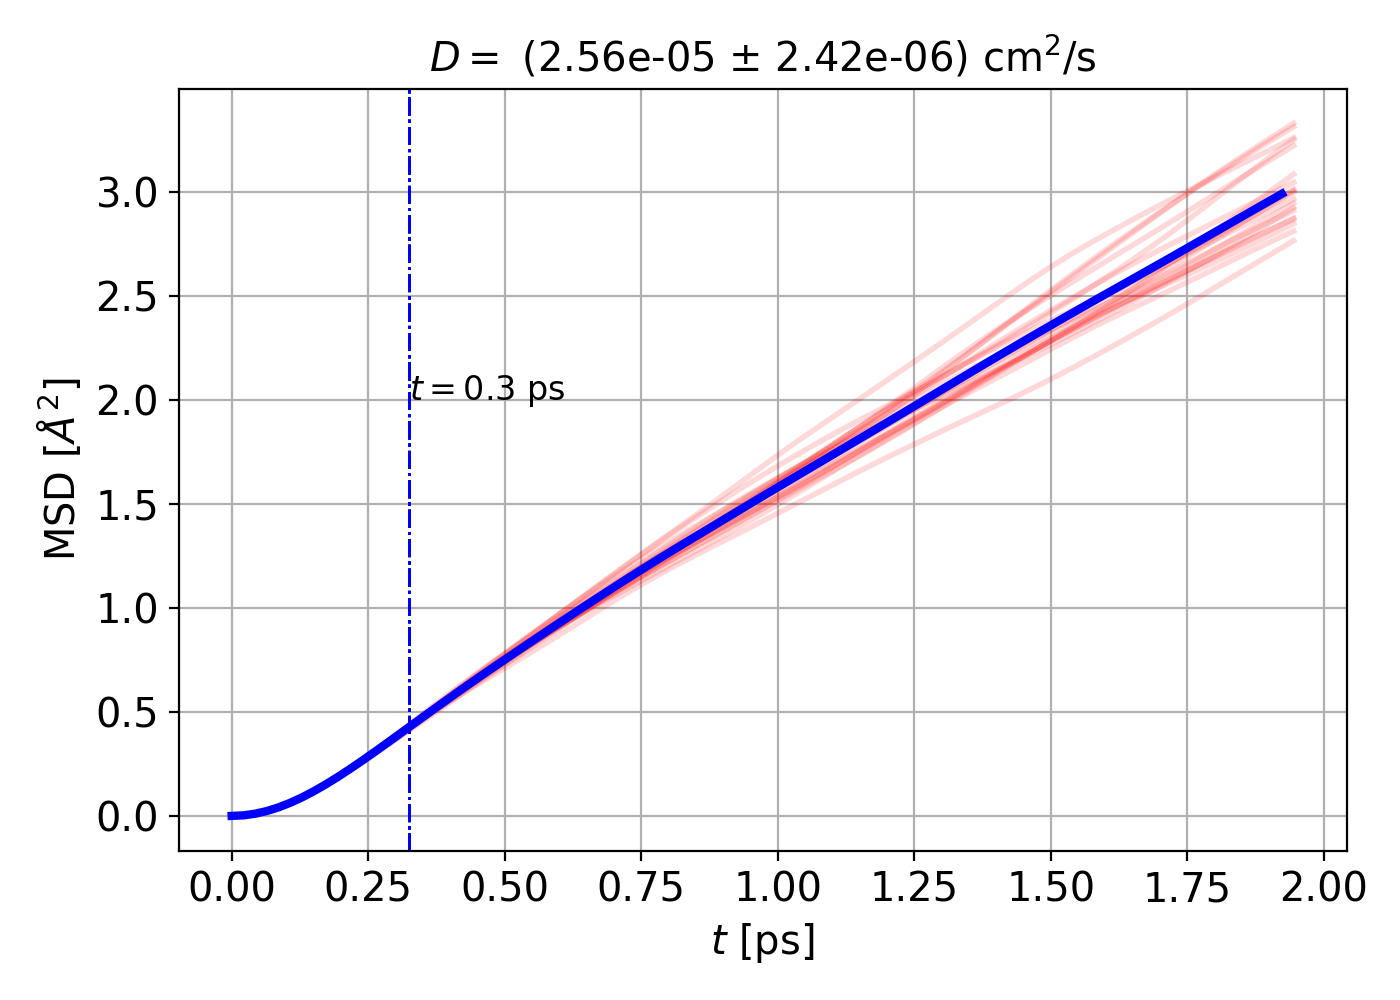
\includegraphics[width=0.9\linewidth]{../task2/results/msdvst}
	\caption{MSD}
	\label{fig:msdvst}
\end{figure}

\begin{figure}
	\centering
	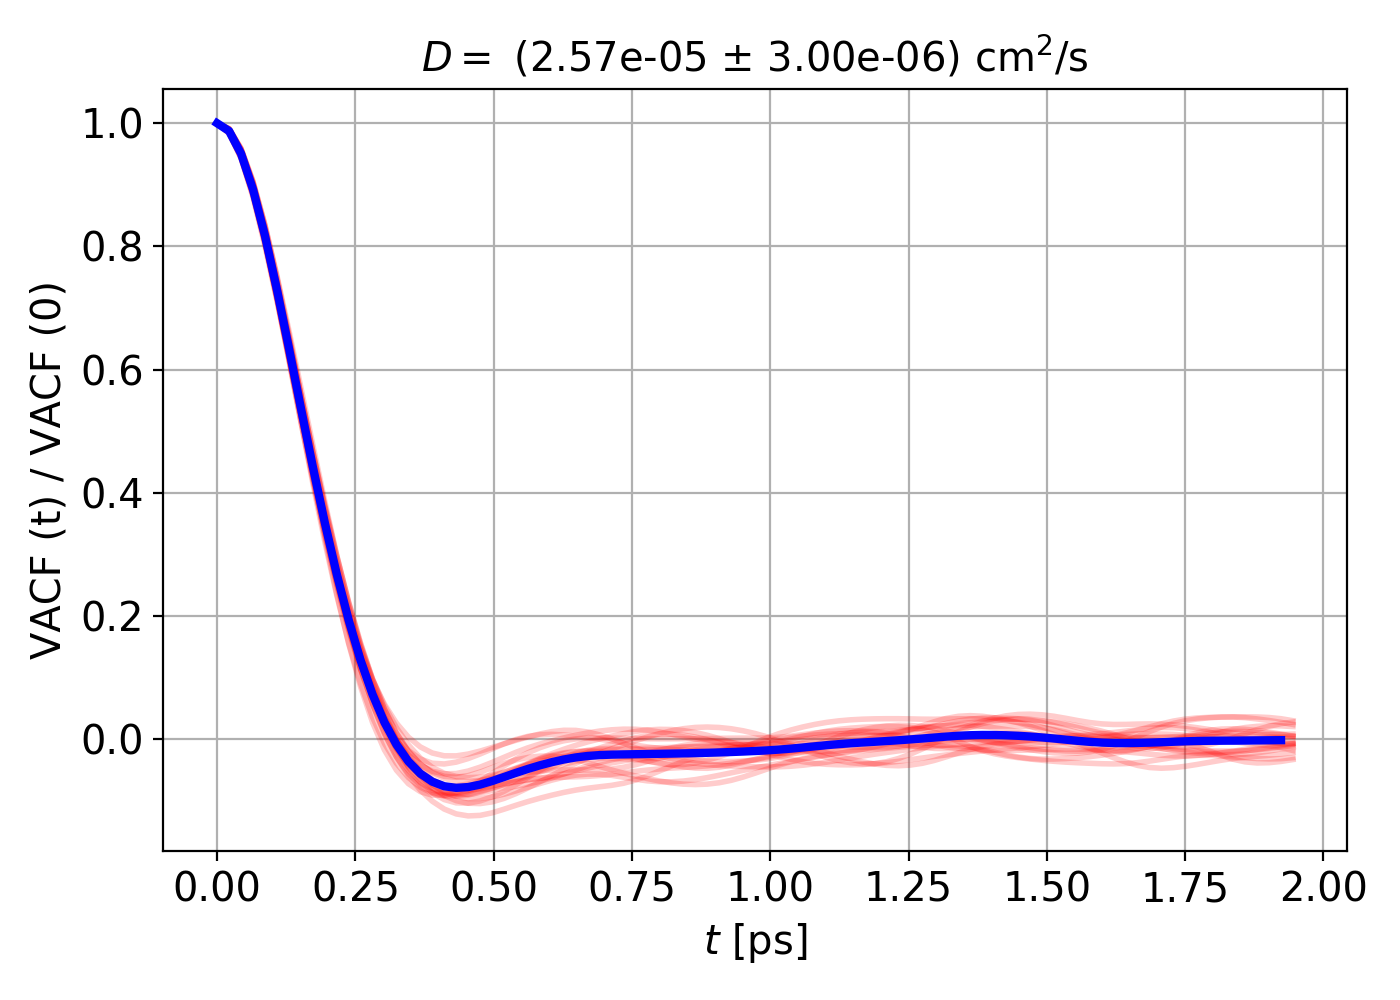
\includegraphics[width=0.9\linewidth]{../task2/results/vacfvst}
	\caption{VACF}
	\label{fig:vacfvst}
\end{figure}



\bibliography{refs}
	

\end{document}
%
% ****** End of file aipsamp.tex ******
